\section{1. Designing and analyzing a typical ET experiment in our field }
Eye-movements provide a fine grain measurement of various levels of language processing.
\parencite[e.g.][]{Tanenhaus_Spivey-Knowlton_Eberhard_Sedivy_1995,Allopenna_1998}. The now classic visual world paradigm (VWP) involves a 2x2 design including a target, competitor(s), and distractor(s) with a variety of possible formats from pictures to words. As seen in figure \ref{fig:core_four}, in the VWP a set of images are displayed on a screen time locked to a point in an audio file (e.g., beaker). Both previewing and delayed presentation of images is common. Ultimately, the specific timing used in a study depends on the design  \parencite[see,][, for a review]{Apfelbaum_Klein-Packard_McMurray_2021}{}{}.  The participant then either needs to select the correct answer based on the audio that they perceived or simply listen and look as the sound stimuli plays (e.g., passive listening). VWP experiments vary widely in what linguistic process is being investigated (e.g., referent prediction, sentence processing, word recognition, phonetic cue integration). However, all VWP experiments carefully control three core constructs (i.e., time, audio stimuli, and visual stimuli) in order to bring meaning to a fourth core construct: eye-fixations. 

\begin{figure}[ht]
    \centering
    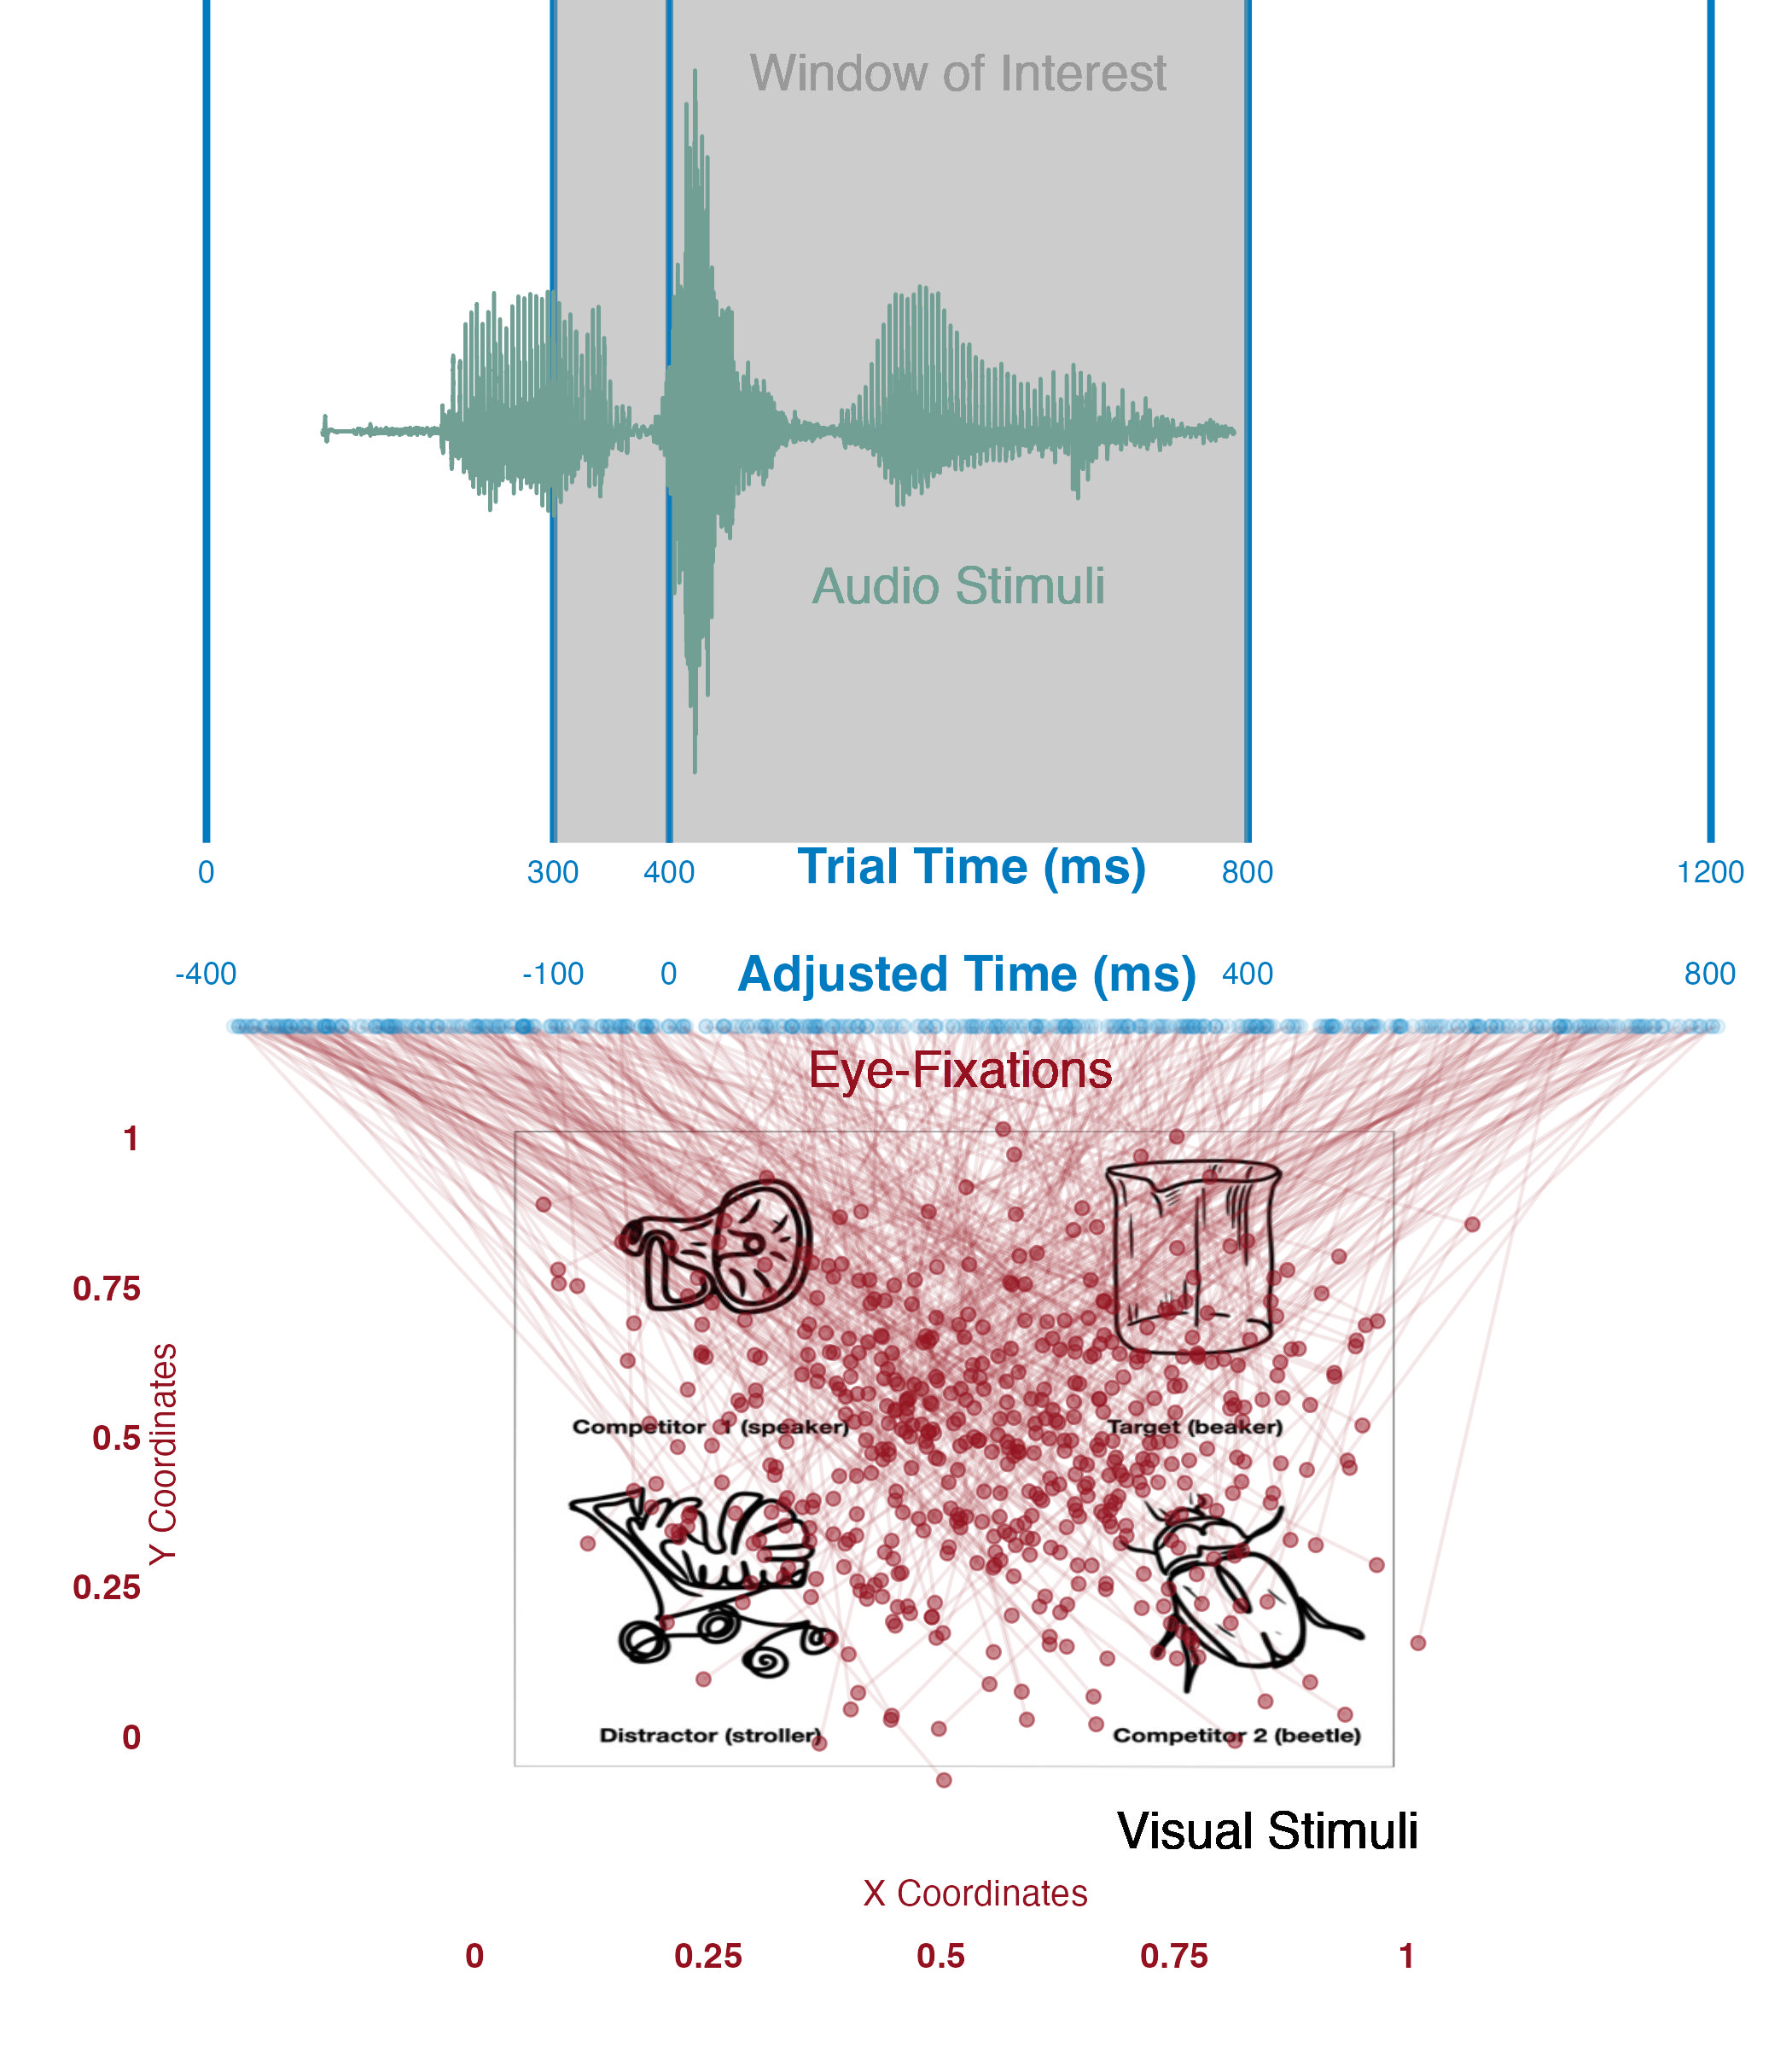
\includegraphics[scale=.182]{figures/Core_four_R.jpeg}
    \caption{A basic illustration of the core four constructs of the VWP. }
    \label{fig:core_four}
\end{figure}

For the remainder of this paper, these "core four" constructs will be used to guide the reader's understanding of how variation in eye-movement behavior can be captured, organized, and analyzed. 

\subsection{The core four of a 2x2 VWP experiment}

\textbf{Time.} Eye-tracking is especially valuable, in part, because it is an online measure that provides the time-course of processing. Time can be measured from the beginning of the trial to the end of the trial. There are two adjustments, however, that are often made to the time variable. First, it typically takes a listener about 200 ms to plan an eye-movement \parencite[][]{Matin_Shao_Boff_1993}. Eye-movements within the first 200 ms are therefore meaningless and researchers typically account for this 200 ms delay by adjusting the analysis. Second, within each trial there exists a window of interest, which is only a portion of the full trial time corresponding to post-audio stimuli presentation. For example, time in which any carrier phrase is presented is typically ignored and time after the start of the target word is examined. As a result, trial time is often converted to an adjusted time.

\textbf{Audio Stimuli.} This is the auditory input a participant receives on each trial. The audio stimuli can be a word, a sentence, or even a non-speech noise. The audio informs the participant about the visual stimuli, often indicating which on screen stimulus is the target or topic of the sentence. The audio stimuli must be carefully locked to time. In this manner, eye-movements are guided by information in the auditory stimuli.   

\textbf{Visual Stimuli:} This is the visual information shown to a participant on each trial. As noted, visual stimuli can be presented at different points in time, either before presentation of audio stimuli (e.g., preview time cite) or simultaneously with the audio stimuli. Visual stimuli are minimally made up of two types: targets and competitors. In the case of four visual stimuli, an additional two visual stimuli include either a second competitor and a single distractor (or two distractors, if a second competitor is not built into the design). Visual stimuli are always counterbalanced across the four quadrants so as to reduce the chances of bias in eye-movements in a particular direction. Note that quadrants are absolute positions on the computer screen (e.g., upper right, upper left, bottom left, bottom right). Figure \ref{fig:Visual_stimuli.png} shows an example. 

\begin{figure}[h]
    \centering
    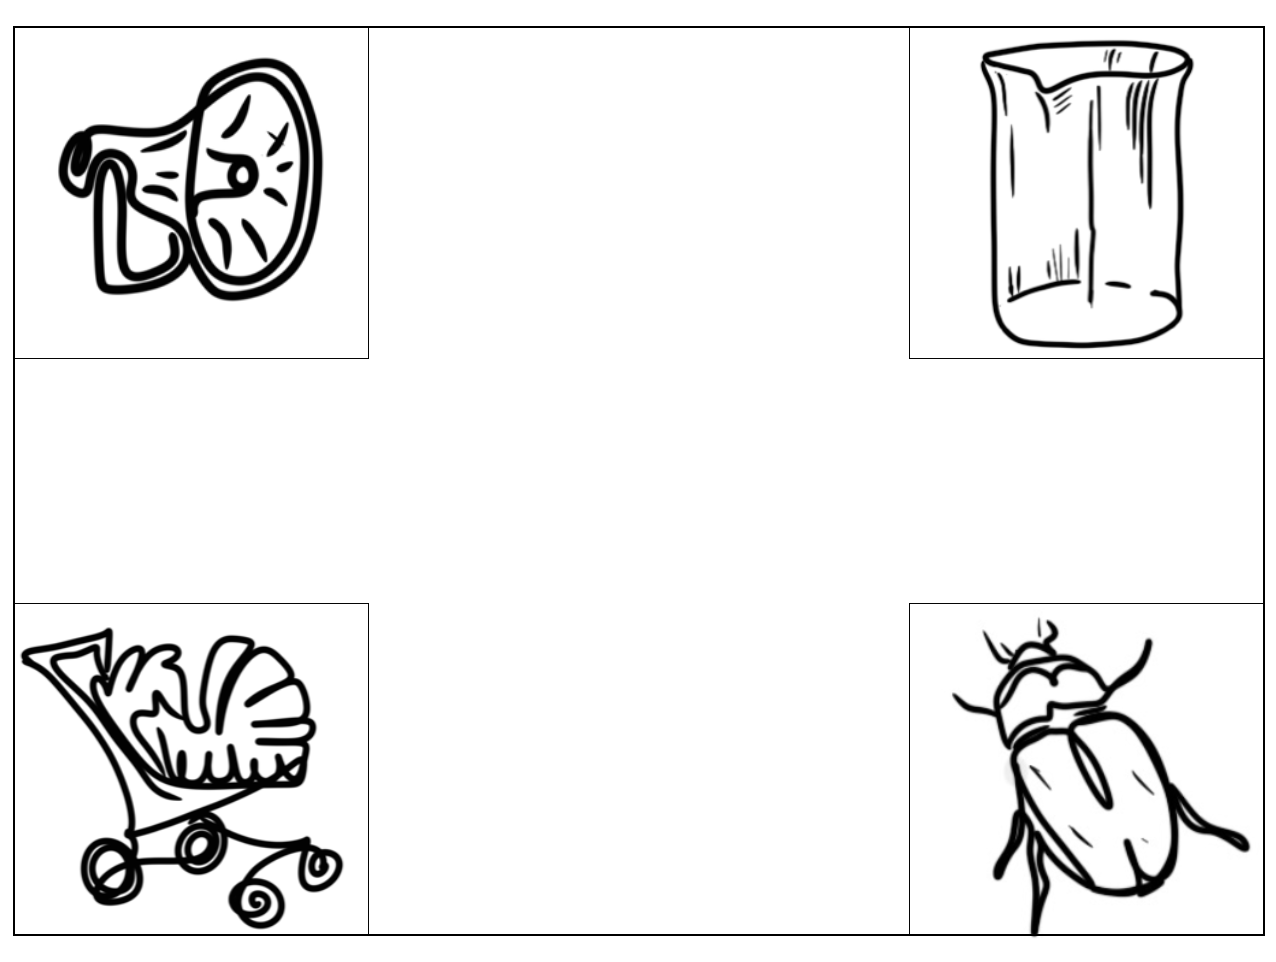
\includegraphics[scale=.35]{figures/Visual_stimuli.png}
    \caption{The four black boxes are surrounding the visual stimuli- Notice visual stimuli are maximally separated}
    \label{fig:Visual_stimuli.png}
\end{figure}

\textbf{Eye-Fixations:} Eye-fixations are time-stamped x- and y- coordinates on the screen that are recorded throughout a trial. In other words, where a participant is looking at a particular time. The rate of recording is a function of the measurements recorded per second (e.g., measuring 1000 times in one second = 1000Hz). Eye-fixations get categorized into absolute positions on the screen (quadrants) and then mapped to visual stimuli. Where a participant is looking over time is informed by the audio stimuli.

\subsection{Building an Eye-tracking Experiment in Gorilla}

Beginning with Task Builder 2, each trial should start with a fixation cross for roughly 200 ms. Next, a simple forced choice task can serve as the foundation of the experiment with four visual stimuli as the choices (see, Gorilla link \footnote{Gorilla link: Experimental ET Tasks: simple forced choice} on OSF \footnote{https://osf.io/a3e5s/?view\_only=bb6015f2526f4a02bdd22dcd7449e9dd}). Audio input comes from the `web audio` zone that plays at the beginning of a specific screen (e.g., delayed). The audio and visual stimuli must have a time locked relationship. The audio stimuli will either provide suggestive hints toward a specific visual stimulus or even explicitly tell the participant which to choose. When building the experiment, it is essential to focus on the timing of the trials, the types of data you want out of the trial, and when the webcam should track eye-fixations. 

In Gorilla, `displays` can be thought of as trials. Each `display` makes up a recursive set of `screens`. `Screens` are made up of `zones`. `Zones` include functionality like (`Response Buttons`,`web audio` and `eye-tracker 2`). The overall timing within a trial is controlled through `screens` with smaller adjustments made within `configuration settings` of each `zone`.  That is, to control the overall relationship between the timing of audio stimuli and visual stimuli (i.e., preview, simultaneous, delayed), web audio should be placed either in the screen before, the screen of, or the screen after the visual stimuli (see example experiments of each in the Gorilla link). From the perspective of 

\begin{figure}[h]
    \centering
    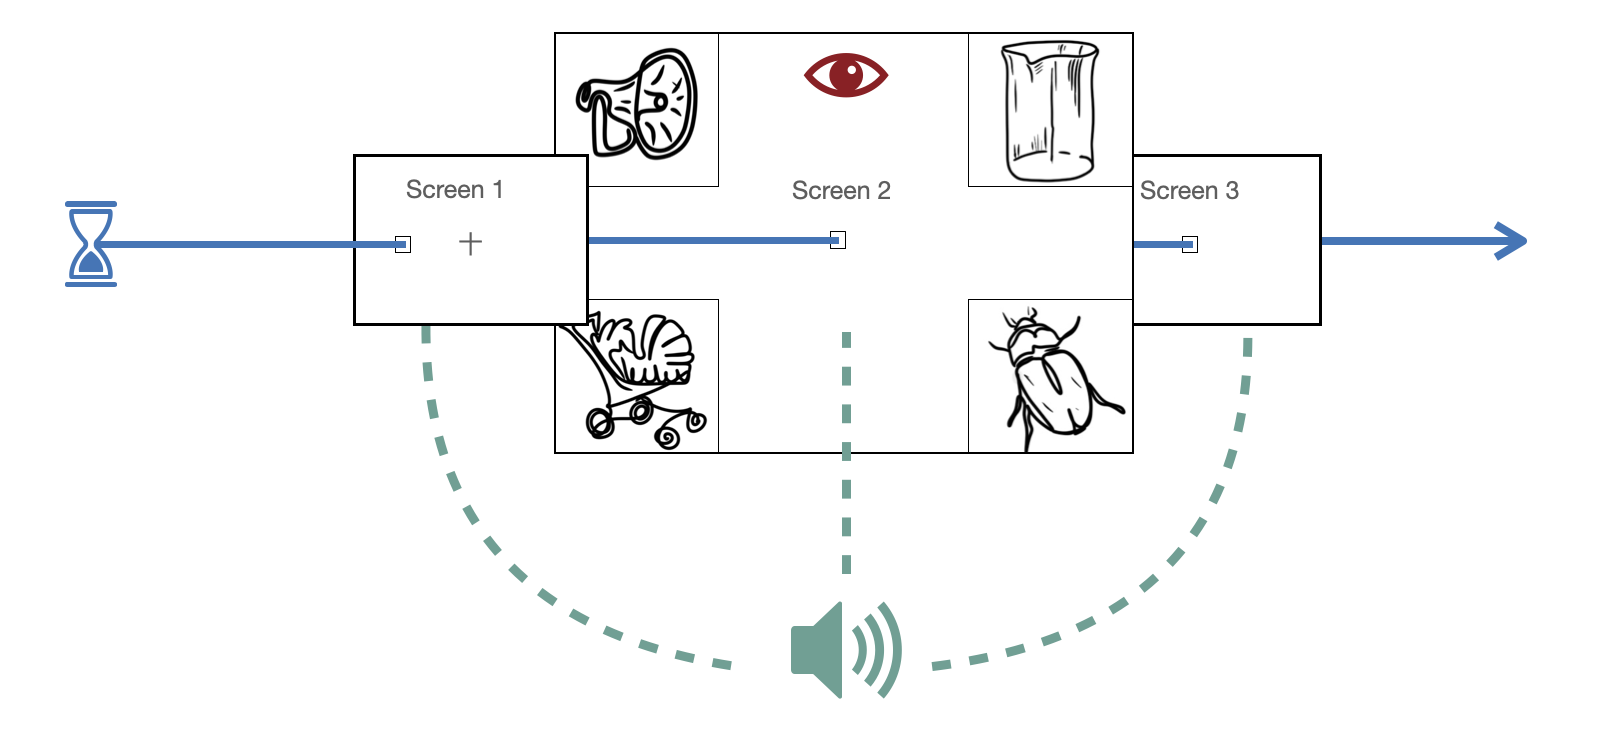
\includegraphics[scale=.5]{figures/Gorilla_work_flow.png}
    \caption{Gorilla Work Flow}
    \label{fig:Gorilla_work_flow}
\end{figure}

\subsection{Gorilla settings}

Eye-tracker 2 from Gorilla has two explicit modes: calibration and recording. Either a five-point or nine-point calibration can be used, with any level set for calibration fail points or repeat calibrations. Nine-point calibration provides a better standard but takes longer and may fail more often. While not fully necessary because of the manner in which  \inlineR{webgazer.js} functions \parencite[e.g.,][]{ Chen_et_al_2001}, it is highly recommended that the researcher calibrate participants at the beginning of the experiment and throughout the experiment \parencite[][]{Prystauka_Altmann_Rothman_2023}. 

The recording screen is used when the visual stimuli begins. All screens you wish to record eye-fixations for should have an eye-tracker module, which will record eye-fixations. Basic eye-tracking data and detailed eye-tracking data are different in that basic data does not provide time course data. Unlike the eye-link 1000 (used in \parencite{Porretta_et_al_2020}), which measures at 1000hz, webcams have variable frame rates that depend on the lighting, participant movement, and the participant's device, which can range between 20hz and 60hz \parencite{Vos_2017}. The raw amount of eye-fixation samples captured per second is maximally 60, but likely much lower in most cases. Additionally, the lighting environment of the participant also has a strong effect on the number of fixations recorded. For example, darker rooms will lead to the camera capturing less eye fixation per second (lower fps). This means that some trials will capture more eye-fixations than other trials. \parencite{} Additionally, the timing of eye-fixations can vary within a trial with non-equal measurements between captured eye fixations. On the aggregate, this means that the eye-fixations being captured starts to drop throughout the trial. This variability in frame rate can be somewhat attenuated by doing in-person eye-tracking with web-gazer but is nonetheless somewhat unavoidable \parencite[e.g.,][]{}{}{}. 

\subsection{Gorilla Data and Tidy Data}

Raw data from a VWP experiment downloaded from Gorilla has two basic parts: behavioral data by node and an \textit{uploads} folder (trial by trial specific data for each participant). This format is not limited to eye-tracking data and is true for any experiment that would need additional trial-specific data (e.g., voice recordings, mouse-tracking) beyond simple behavioral responses (e.g., reaction time, accuracy). Behavioral data will include all selections and timing of those selections (e.g., reaction time, condition, trial order). However, the additional uploads folder will contain trial by trial eye-fixation data that is paired with within trial trial-time. A simplified example of this is shown in figure \ref{fig:data_structure}. The amount of behavioral data sheets has a direct relationship with the number of experimental (and/or questionnaire) nodes in your experiment. While it depends on your design, if counterbalancing audio stimuli by conditions so that participants do not hear the same audio from two speakers, then each of these will also have their own node. That is, if you were to have four counterbalanced stimuli spreadsheets in your experiment design then you will have four raw behavioral data sheets, one from each of these nodes. However, the number of spreadsheets in the upload data folder will depend on how many participants and trials you have. For example, if you have 60 participants who finish 50 trials, you will have a total of 3,000 eye-tracking data sheets (50X60) that reference the behavior trials in your four behavioral data sheets.

\begin{figure}[ht]
    \centering
    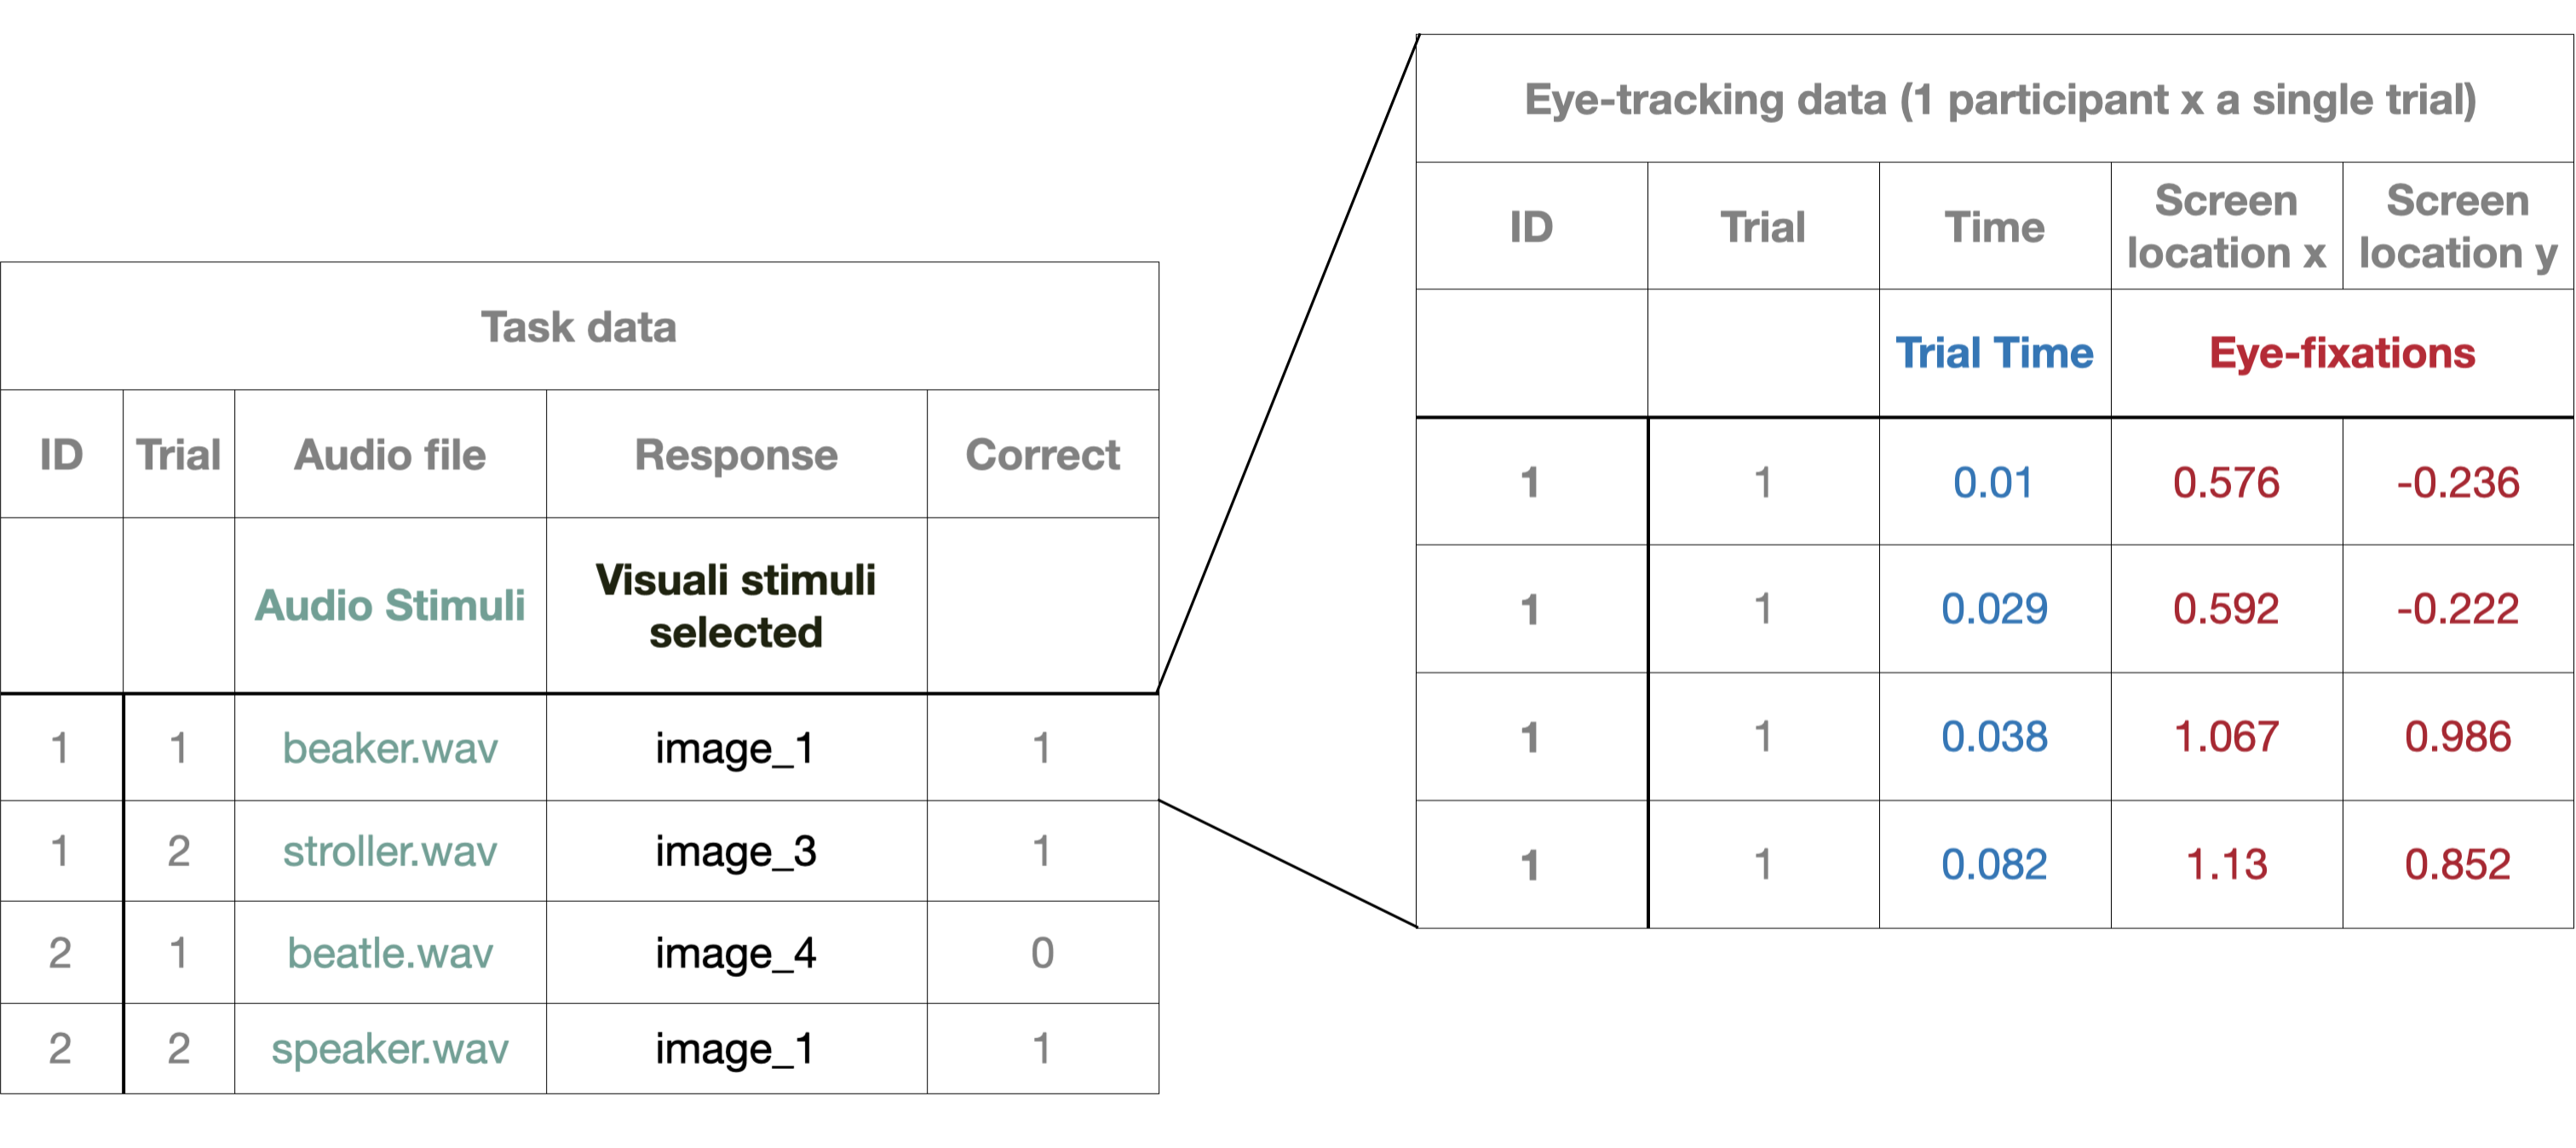
\includegraphics[scale=.3]{figures/data_structure.png}
    \caption{Behaviorial data (left) and trial by trial eye-tracking data (right)-\textit{upfloads} data. Colors match figure \ref{fig:core_four} layout for ease.}
    \label{fig:data_structure}
\end{figure}

The raw data that Gorilla provides is maximally informative to enable a variety of experiments and analyses to be done. However, this also means that the data is messy. Tidy data is data where each column refers to a single variable (e.g., audio stimuli) and each row is exactly one observation (e.g., bird.wav). However, what one observation means varies depending on your question. For example, if you are examining questionnaire data, it is likely that each row should have the answer to many questions, where each question is a single column. However, if you are looking at behavioral data then each row shows a different trial for each participant with their response as a single observation. The ways that data can be thought of for tidying will be shown in examples below.


